%% ----------------------------------------------------------------
%% Thesis.tex -- MAIN FILE (the one that you compile with LaTeX)
%% ---------------------------------------------------------------- 

% Set up the document
\documentclass[letter, 11pt, oneside]{Thesis}  % Use the "Thesis" style, based on the ECS Thesis style by Steve Gunn
\graphicspath{Figures/}  % Location of the graphics files (set up for graphics to be in PDF format)

% Include any extra LaTeX packages required
\usepackage[square, numbers, comma, sort&compress]{natbib}  % Use the "Natbib" style for the references in the Bibliography
\usepackage{verbatim}  % Needed for the "comment" environment to make LaTeX comments
\usepackage{vector}  % Allows "\bvec{}" and "\buvec{}" for "blackboard" style bold vectors in maths
\hypersetup{urlcolor=blue, colorlinks=true}  % Colours hyperlinks in blue, but this can be distracting if there are many links.

%% ----------------------------------------------------------------
\begin{document}
\frontmatter      % Begin Roman style (i, ii, iii, iv...) page numbering

% Set up the Title Page
\title  {A really long thing that I wrote once}
\authors  {
            {Steven Chien}
            }
\addresses  {\groupname\\\deptname\\\univname}  % Do not change this here, instead these must be set in the "Thesis.cls" file, please look through it instead
\date       {\today}
\subject    {}
\keywords   {}

\maketitle
%% ----------------------------------------------------------------

\setstretch{1.3}  % It is better to have smaller font and larger line spacing than the other way round

% Define the page headers using the FancyHdr package and set up for one-sided printing
\fancyhead{}  % Clears all page headers and footers
\rhead{\thepage}  % Sets the right side header to show the page number
\lhead{}  % Clears the left side page header


%% ----------------------------------------------------------------
% Declaration Page required for the Thesis, your institution may give you a different text to place here
\pagestyle{empty}

\vspace*{\fill}

I hereby declare that this Independent work represents my own work in accordance with University regulations.
 
\hfill 
 
Signed: \hrulefill

\textbf{Steven Chien}

\clearpage  % Declaration ended, now start a new page

%% ----------------------------------------------------------------

% The Abstract Page
\addtotoc{Abstract}  % Add the "Abstract" page entry to the Contents
\abstract{
\addtocontents{toc}{\vspace{1em}}  % Add a gap in the Contents, for aesthetics

Much of the restrictions on quantum secret sharing schemes are derived from the no-cloning theorem. In this paper, we consider the implications of implementing quantum secret sharing schemes using two or more identical copies of the same secret....

% keep going boy
}

\clearpage  % Abstract ended, start a new page
%% ----------------------------------------------------------------

\setstretch{1.3}  % Reset the line-spacing to 1.3 for body text (if it has changed)

% The Acknowledgements page, for thanking everyone
\acknowledgements{
\addtocontents{toc}{\vspace{1em}}  % Add a gap in the Contents, for aesthetics

I would like to thank Mark Zhandry for all of his help in advising me for this thesis. 

\null
\vfill

\textit{``Mama told me save that money -- bank accounts -- don't spend that bread.''}

\begin{flushright}
A\$AP Ant
\end{flushright}

}
\clearpage  % End of the Acknowledgements
%% ----------------------------------------------------------------

\pagestyle{fancy}  %The page style headers have been "empty" all this time, now use the "fancy" headers as defined before to bring them back


%% ----------------------------------------------------------------
\lhead{\emph{Contents}}  % Set the left side page header to "Contents"
\tableofcontents  % Write out the Table of Contents

%% ----------------------------------------------------------------
\lhead{\emph{List of Figures}}  % Set the left side page header to "List if Figures"
\listoffigures  % Write out the List of Figures

%% ----------------------------------------------------------------
%\lhead{\emph{List of Tables}}  % Set the left side page header to "List of Tables"
%\listoftables  % Write out the List of Tables

%% ----------------------------------------------------------------
\setstretch{1.5}  % Set the line spacing to 1.5, this makes the following tables easier to read
\clearpage  % Start a new page
\lhead{\emph{Abbreviations}}  % Set the left side page header to "Abbreviations"
\listofsymbols{ll}  % Include a list of Abbreviations (a table of two columns)
{

\textbf{QSS} & \textbf{Q}uantum \textbf{S}ecret \textbf{S}haring \\

\textbf{QTS} & \textbf{Q}uantum \textbf{T}hreshold \textbf{S}cheme \\

\textbf{QECC} & \textbf{Q}uantum \textbf{E}rror \textbf{C}orrecting \textbf{C}odes \\

\textbf{MSP} & \textbf{M}onotone \textbf{S}panning \textbf{P}rograms \\

}
\clearpage  %Start a new page
\lhead{\emph{Symbols}}  % Set the left side page header to "Symbols"
\listofnomenclature{lll}  % Include a list of Symbols (a three column table)
{
% symbol & name \\
$\mathcal{D}$ & dealer \\
$\mathcal{S}$ & secret \\
$\Gamma$ & access structure \\
$\ket{\Psi}$ & quantum state \\
$U$ & unitary operator \\
$H$ & hypergraph \\
$G$ & graph \\ 
$L(G)$ & line graph \\ 
$G^c$ & complement of graph \\ 
}
%% ----------------------------------------------------------------
% End of the pre-able, contents and lists of things
% Begin the Dedication page

\setstretch{1.3}  % Return the line spacing back to 1.3

\addtocontents{toc}{\vspace{2em}}  % Add a gap in the Contents, for aesthetics


%% ----------------------------------------------------------------
\mainmatter	  % Begin normal, numeric (1,2,3...) page numbering
\pagestyle{fancy}  % Return the page headers back to the "fancy" style

% Include the chapters of the thesis, as separate files
% Just uncomment the lines as you write the chapters

\chapter{Introduction}

Secret sharing is a cryptographic procedure by which we take some sensitive data or a "secret" and distribute it among individual parties in such a way that access to the secret requires sufficiently large subsets of those parties to come together. Applications of these schemes are numerous, but some examples include giving a group of bank executives  access to a vault, requiring multiple officials to launch nuclear warheads, and creating secure voting procedures for a board of directors. In general, a secret sharing scheme is useful in a group of people where there is mutual distrust between its members, but they are forced to cooperate, either because there is information that is too sensitive for one person to access, or power must be distributed among its members in some way.

The moment that quantum computers become viable ways to store and perform operations on information, quantum computing algorithms and quantum cryptography will become extremely important. And so, thinking about quantum implementations of classical cryptographic procedures is a necessary and important exercise. Since 1999, researchers have been thinking about the implementation of secret sharing schemes in quantum computers. Hillery, Bu\u{z}ek, and Berthiaume presented one of the first schemes that involves using GHZ states to split quantum information into two parts such that both are necessary to recover the original information \cite{Hillery_1999}. Gottesman, Cleve, Lo use quantum error correcting codes to implement both threshold schemes and schemes with general access structures \cite{Cleve_1999}. Smith presents a construction for general access structures using monotone span programs. Later, Gottesman proves several important theorems regarding the realizability of quantum secret sharing schemes \cite{singh_assisted_2004}.

One of the main limitations of quantum secret sharing schemes come about as a consequence of the \textit{no-cloning theorem}. This theorem states that we cannot make a copy, or a clone, of an unknown quantum state. As we will later discuss, this restriction presents several practical limitations for applying secret sharing schemes to quantum computing. Therefore, the goal of this thesis is to explore ideas that will allow us to implement quantum threshold schemes that would otherwise be impossible to realize due to the no-cloning theorem. This idea is not new. Singh and Srikanth explore an idea that involves keeping a certain number of quantum shares with the dealer, and they show that they are able to completely remove the restriction imposed by the no-cloning theorem. 

In this paper, we present a new approach that achieves a similar goal of loosening the restriction of the no-cloning theorem. In Chapter 2, we will present relevant background for both classical and quantum secret sharing (QSS schemes). We will do things like prove the no-cloning theorem, and establish necessary quantum computing preliminaries. We will also bring in some other theory that will become useful in our analysis, such as some definitions and results from graph theory. In Chapter 3, we present our approach to circumventing the no-cloning theorem, and begin to reason about quantum threshold schemes (QTS) using multiple copies of the same state. In Chapter 4, we take our approach and prove some general claims about it. One of these claims characterizes the quantum threshold schemes that our new formulation can realize. Finally, we present a short corollary that provides a closed-form solution for the minimum number of shares that must reside with the dealer in Singh and Srikanth's \textit{Assisted Quantum Threshold Scheme} by using a well known result from graph theory. In the final chapter, we discuss the implications of our findings and explore possible future work. % Introduction

\chapter{Background}

\section{Classical Secret Sharing}

In this section we will describe secret sharing schemes and talk about some of its properties and definitions. A secret sharing scheme allows some \textit{secret} $\mathcal{S}$ to be divided into shares and distributed by some \textit{dealer} $\mathcal{D}$ to a set of \textit{participants} $\mathcal{P}$. Each secret sharing scheme has a corresponding \textit{access structure} denoted by $\Gamma$. $\Gamma$ defines the set of \textit{authorized subsets} of participants that have access to the secret. A subset of participants $A \in \Gamma$ should be able to reconstruct the original secret, but a a set $B \notin \Gamma$ should have \textbf{no} information about the secret, in the sense that all possible values of the secret are equally likely. Let us present some more formalized definitions:

\theoremstyle{definition}
\begin{definition}{Access Structure.}
    An \textbf{access structure} is often denoted as $\Gamma$. An access structure specifies the set of all authorized subsets of users that are able to recover the secret.
\end{definition}

\theoremstyle{definition}
\begin{definition}{Monotonic Access Structure.}
    An access structure $\Gamma$ is \textbf{monotonic} if $B \in \Gamma$ and $B \subseteq C$ implies $C \in \Gamma$.
\end{definition}

This is a particularly useful definition. Essentially, if some subset satisfies the access structure, then larger groups that contain that subset must also satisfy the access structure. We will see later on that the property of monotonicity for an access structure leads to strong claims within quantum secret sharing schemes. For now, and for the sake of simplicity, we will assume that our access structures are monotone. When we describe an access structure, we will do so using its \textbf{minimal} authorized subsets. These are the subsets $A_0, A_1... \in \Gamma$ whose proper subsets are not in $\Gamma$. The set of minimal authorized subsets completely defines an access structure. 

\theoremstyle{definition}
\begin{definition}{Threshold Scheme.}
    A \textbf{$(t,n)$-threshold secret sharing scheme} is a secret sharing scheme among $n$ individuals such that at least $t$ of those individuals must work together to access the secret. The access structure for this scheme is composed of every subset of $\mathcal{P}$ of size $t$.
\end{definition}

We say that $A$ is authorized if $A \in \Gamma$. So, for our $(t,n)$ threshold scheme defined above, the access structure can be defined more formally as such: $\Gamma = \{A | A \subseteq \mathcal{P} , |A| = t\}$.

A more concrete example of an access structure for a set of participants $\mathcal{P} = \{p_1,p_2,p_3\}$ might be $\Gamma = \{p_1p_2,p_2p_3,p_3p_1\}$. This access structure describes a $(2,3)$ threshold scheme.

In 1979, Shamir developed one of the first implementations for a perfect threshold scheme based on polynomial interpolation \cite{shamir-whisper}. His scheme is a $(t,n)$-threshold secret sharing scheme. The scheme works as so. First, encode the secret as some number. Then, generate a $t-1$ degree polynomial. For each of the $n$ participants, generate a pair $i, p(i)$, where $i \in [1, \cdots, n]$, and distribute one such pair to each participants. Then, if $t$ or more participants get together and share their points, they can reconstruct the unique polynomial $p$ that generated those points, and $p(0)$ reveals the secret. Note that, having only $t-1$ or fewer points gives no information about the secret, because there would be infinitely many polynomials of degree $t-1$ passing through those number of points.

\section{Quantum Computing Preliminaries}

The basic unit of information in a quantum computer is the qubit, or the "quantum bit". A qubit is represented as a quantum state:

% flesh out this definition
\begin{align*}
    \ket{\psi} &= \sum_{i=1}^n \alpha_i\ket{i} \\ 
\end{align*}

% talk about a quantum operation

One of the most important theorems that has a large effect on quantum computing algorithms is the \textbf{no-cloning theorem}. Here, we present the no-cloning theorem with proof referencing Mermin's 2007 text \cite{merlin}.

\begin{theorem}{No cloning theorem}
    \label{no-cloning-thm}
    Given an unknown, arbitrary quantum state $\psi$, there is no valid operator $U$ that can create an identical copy of this state. More formally there exists no operator such that $U(\ket{\psi} \ket{0}) = \ket{\psi}\ket{\psi}$.
\end{theorem}

\begin{proof}
    Assume for the sake of contradiction that there is such an operator. Then $U(\ket{\psi} \ket{0}) = \ket{\psi}\ket{\psi}$ and $U(\ket{\phi} \ket{0}) = \ket{\phi}\ket{\phi}$, for arbitrary quantum states $\ket{\psi}, \ket{\phi}$. Then:
    
    \begin{align*}
        U(\alpha \ket{\psi} + \beta \ket{\phi})\otimes\ket{0} &= (\alpha \ket{\psi} + \beta \ket{\phi})\otimes (\alpha \ket{\psi} + \beta \ket{\phi}) \\ 
        &= \alpha^2\braket{\phi|\phi} + \beta^2\braket{\psi|\psi} + \alpha \beta \braket{\phi|\psi} + \alpha \beta \braket{\psi|\phi} \numberthis \label{no-clone-1}\\ 
    \end{align*}
    
    But by linearity, we also have:
    
    \begin{align*}
        U(\alpha \ket{\psi} + \beta \ket{\phi})\otimes\ket{0} &= \alpha U \ket{\psi}\ket{0} + \beta U \ket{\phi}\ket{0} \\ 
        &= \alpha \ket{\psi}\ket{\psi} + \beta \ket{\phi}\ket{\phi} \numberthis \label{no-clone-2}\\ 
    \end{align*}
    
    Equation \ref{no-clone-1} and equation \ref{no-clone-2} can only be the same if one of $\alpha$ or $\beta$ is equal to 0, which contradicts the assumption that $\ket{\psi}, \ket{\phi}$ are arbitrary.
\end{proof}

\theoremstyle{remark}
\begin{remark}
    Note that the theorem statement can also be made with any state $\ket{e}$ instead of $\ket{0}$. What is important is that there is no unitary operator that acts as a "general purpose copier", where the relation between the state that is to be copied and the state that is being overwritten is arbitrary. For example, it would be easy to create an operator that can copy a state $\ket{\phi}$ if we know for a fact that the state is either $\ket{0}$ or $\ket{1}$.
\end{remark}

\section{Quantum Secret Sharing}

A quantum secret sharing scheme is the quantum analogue of a (classical) secret sharing scheme. In these schemes, the secret to be shared takes the form of a quantum state $\ket{\psi}$. This idea was first introduced by Hillery et al. in 1998 \cite{Hillery_1999}. In their paper, they give an example of using GHZ states to implement a $((2,3))$-threshold quantum secret sharing scheme. This was then extended by the work of Cleve, Gottesman, and Lo \cite{Cleve_1999}. In their paper, they introduce the idea of a quantum access structure, and propose implementation for a general threshold schemes.

\theoremstyle{definition}
\begin{definition}{Quantum Threshold Scheme.}
    A quantum threshold scheme (QTS) is a threshold secret sharing scheme applied to a quantum secret. This secret is denoted as $\ket{\psi}$. As in the classical case, we take a quantum secret and divide it into shares to distribute among a set of individuals. We will denote a QTS among $n$ individuals with a threshold of $t$ as $((t,n))$, using double parentheses to denote that the scheme is quantum.
\end{definition}

\begin{theorem}
    \label{qss-disjoint}
    A QSS scheme exists for a general access structure $\Gamma$ only if for every $A_1, A_2 \in \Gamma$, $A_1 \cap A_2 \neq \emptyset$.
\end{theorem}

\begin{proof}
    Let's assume, for the sake of contradiction, that there exist two disjoint subsets such that each recover the secret. Then, we would have two copies of the quantum state, which violates Theorem \ref{no-cloning-thm}. 
\end{proof}

\begin{theorem}
    \label{qts}
    A QTS $((t,n))$ exists only if $t > \frac{n}{2}$.
\end{theorem}

\begin{proof}
    This theorem is a direct result of Theorem \ref{qss-disjoint}. If $t \leq \frac{n}{2}$, then there would exist at least two authorized subsets that are disjoint. 
\end{proof}

Note that this theorem does not guarantee the existence of a QTS if this inequality of the threshold is met, only that one cannot exist if the inequality is not met. However, we can indeed prove stronger claims. In 2000, Gottesman showed that a quantum secret sharing scheme exists for an access structure $\Gamma$ as long as $\Gamma$ is monotone and Theorem \ref{qss-disjoint} is satisfied \cite{Gottesman_2000}:

\begin{theorem}
    \label{monotone-gamma}
    A quantum secret sharing scheme exists for an access structure iff the access structure is monotonic and the no-cloning theorem is not violated.
\end{theorem}

As we can see, the no-cloning theorem imposes most of the limitations on realizable QSS schemes. In \cref{ch3}, we will explore some ideas that have the potential to relax the constraints on our QSS schemes. 

 
\section{Hypergraph Formulation}

Access structures lend themselves naturally to graphical representations. One way of representing access structures is using a \textit{hypergraph}.

\theoremstyle{definition}
\begin{definition}{Hypergraph.}
    A hypergraph $H$ is a pair $(V,E)$ that specify a set of vertices $V$ and a set of hyperedges $E$. A hyperedge is the extension of a normal edge where the edge can have any number of non-zero endpoints, up to the number of vertices in the graph.
\end{definition}

\theoremstyle{definition}
\begin{definition}{Hypercycles.}
    A hypercycle $H$ is a hypergraph $H = (V,E)$ where there exists an ordering of hyperedges: $(E_1, E_2, \cdots, E_{m-1})$ such that $E_{i} \cap E_{(i+1) m o d m} \neq \emptyset$ for $i = 1,2,\cdots,m-1$.
\end{definition}

\theoremstyle{definition}
\begin{definition}{Hyperstars.}
    A hyperstar is a hypergraph $H = (V,E)$ where the intersection of all the hyperedges $\bigcap_{E_{i} \in E} E_{i} \neq \varnothing$.
\end{definition} % Background Theory 

\chapter{An Augmented Quantum Threshold Scheme}
\label{ch3}

As we have shown above, one of the main limitations of QC comes from the no-cloning theorem. The first idea we pose attempts to circumvent this limitation. 

If we begin with two identical copies of a quantum state, then what does this do, if anything, to change the limitations surrounding the value of $t$ with respect to $n$? What if we have $k$ copies? What schemes are realizable in this new formulation? In this section, we will explore the properties of such a scheme. We will call this an augmented quantum threshold scheme. Let us formalize this idea and explore its consequences below:

\theoremstyle{definition}
\begin{definition}{Augmented Quantum Threshold Scheme.}
    \label{defn:augmented-qts}
     This is a QTS that assumes that we being with $k$ identical copies of a quantum state prepared in advance. As with the normal QTS, we need at least $t$ individuals to come together to recover the secret quantum state. We will denote an augmented QTS as $((t,n,k))$.
\end{definition}

\section{Preliminary thoughts}

Let's consider the case of $k=2$. If we consider just the consequences of the no-cloning theorem, an extension of \thmref{thm:qss-disjoint} can be posed as follows:

\begin{theorem}
    \label{thm:three-authorized}
    In any valid $((t,n,2))$ scheme, any three authorized subsets cannot be pair-wise disjoint.
\end{theorem}

And a generalization to the case with $k$ identical copies:

\begin{theorem}
    \label{thm:k-authorized}
    In any valid $((t,n,k))$ scheme, any $k+1$ authorized subsets cannot be pair-wise disjoint.
\end{theorem}

We can also extend \thmref{thm:qts} in a similar manner:

\begin{theorem}
	\label{thm:qts2}
	A QTS $((t,n, 2))$ exists only if $t > \frac{n}{3}$.
\end{theorem}

\begin{theorem}
	\label{thm:qtsk}
	A QTS $((t,n, k))$ exists only if $t > \frac{n}{k+1}$.
\end{theorem}

Each of the proofs of these theorems are almost identical to that of \thmref{thm:qss-disjoint}. However, these theorems only present to us what schemes are not immediately ruled out by the no-cloning theorem. Figuring out methods of realizing these schemes is a different question. It is not immediately obvious that Gottesman's \thmref{thm:monotone-gamma} applies to augmented threshold schemes.

\section{A Union of Access Structures Approach}

The simplest case that is non-trivial is to consider a $((2,4,2))$ scheme. Using 2 identical copies of a quantum state, is it possible to implement a scheme among 4 individuals such that only 2 or more people need to come together to recover the secret? The answer is yes.

The strategy that we will use will employ a strategy where we take the union of two valid access structures, each using only one quantum state each. Let the two copies of our quantum secret be $\ket{\psi_1}, \ket{\psi_2}$, and let the participants be labeled $p_1, p_2, p_3, p_4$. \fref{fig:2-4-2} shows how we implement the scheme. Each node corresponds to one participant, and the blue edges denote authorized subsets of size 2 that are a part of the access structure $\Gamma_1$ of $\ket{\psi_1}$. Red edges correspond to $\Gamma_2$, which is the access structure of $\ket{\psi_2}$.


\begin{figure}[ht]
	\begin{center}
        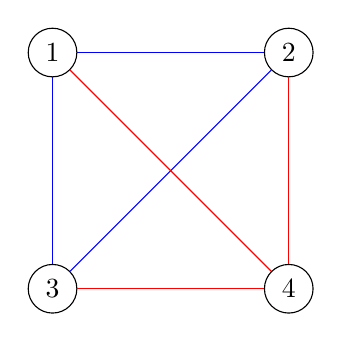
\begin{tikzpicture}[scale=3,auto=left,every node/.style={circle,draw,fill=white}]
          \node (n1) at (0,1) {1};
          \node (n2) at (1,1) {2};
          \node (n3) at (0,0) {3};
          \node (n4) at (1,0) {4};
          
          \draw [blue] (n1) -- (n2);
          \draw [blue] (n3) -- (n2);
          \draw [blue] (n1) -- (n3);
          \draw [red] (n1) -- (n4);
          \draw [red] (n2) -- (n4);
          \draw [red] (n3) -- (n4);
        \end{tikzpicture}
	\end{center}
	\caption{An image of the access structure for a $((2,4,2))$ threshold scheme, using two copies of the quantum secret.}
	\label{fig:2-4-2}
\end{figure}


The scheme is as follows: $\Gamma_1 = \{p_1p_2,p_2p_3,p_3p_1\}$ and $\Gamma_2 = \{p_1p_4,p_2p_4,p_3p_4\}$. Observe that each access structure satisfies \thmref{thm:qss-disjoint}. By \thmref{thm:monotone-gamma}, a $((2,4,2))$ scheme exists.

\subsection{A Better Graphical Representation}

How can we generalize this strategy? Notice that in the case of the $((2,4,2))$ scheme, we need the union $\Gamma_1 \cup \Gamma_2$ to consist of all subsets of size 2. Each of these access structures must satisfy Theorem \ref{thm:qss-disjoint}. So, in general, a $((t,n,k))$ scheme is realizable if we can take all subsets of size $t$ of the $n$ participants and divide them into $k$ groups, where each group consists of an access structure that satisfies Theorem \ref{thm:qss-disjoint}. 

Let's dive deeper into augmented threshold schemes of the form: $((t,n,2))$. What would be useful for us is a representation of this problem that allows us to better reason about the authorized subsets contained in the access structures. The formulation we use in \fref{fig:2-4-2} is a natural one: where each node represents a participant, and the edges represent authorized subsets. However, we run into the problem where we can only properly represent authorized subsets of size 2.

So, instead of representing the participants as vertices and the authorized subsets as edges, we take inspiration from Singh and Srikanth's \cite{singh_assisted_2004} AS graph representation, which we defined in \defref{defn:access-structure-graph}. We \textbf{make each authorized subset a vertex}, and have the edges denote some relationship between the authorized sets. However, we make one modification from their representation. Instead of having an edge between any two authorized sets that overlap, we place an edge between them if they \textbf{do not overlap}. In other words, this is the \textit{complement} of the AS graph.

\begin{definition}{Access Structure Graph Complement.}
    \label{defn:access-structure-graph-complement}
	We define an \textbf{access structure graph} of $\Gamma$ to be the graph $G = (V,E)$, where there is a vertex $v \in V$ for each authorized subset $A \in \Gamma$. The edgeset $E$ contains an edge between each pair of vertices if their corresponding authorized subsets are disjoint.
\end{definition}

The access structure graph complement for \fref{fig:2-4-2} is shown in \fref{fig:2-4-2-graph}. Later in this section, we will explore why using the complement of the AS graph can be beneficial to us:

\begin{figure}[H]
    \centering
	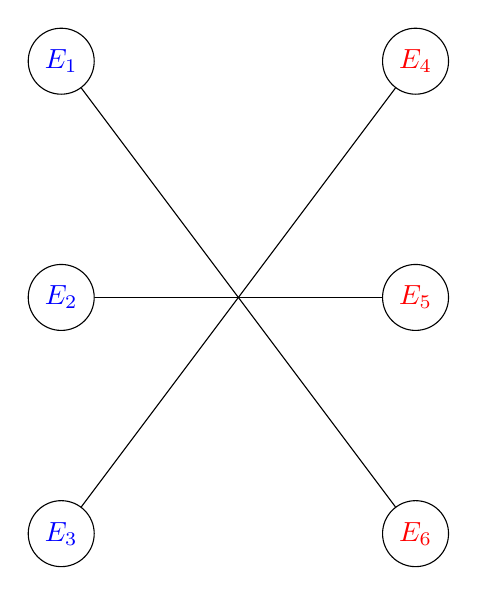
\begin{tikzpicture}[scale=3,every
	node/.style={circle,fill=white}]
      \node [draw,text=blue] (n1) at (0,3)   {$E_1$};
      \node [draw,text=blue] (n2) at (0,2)   {$E_2$};
      \node [draw,text=blue] (n3) at (0,1)   {$E_3$};
      \node [draw,text=red] (n4) at (1.5,3) {$E_4$};
      \node [draw,text=red] (n5) at (1.5,2) {$E_5$};
      \node [draw,text=red] (n6) at (1.5,1) {$E_6$};
      
      \draw [black] (n1) -- (n6);
      \draw [black] (n3) -- (n4);
      \draw [black] (n2) -- (n5);
    \end{tikzpicture}
	\caption{The access structure graph representation for a $((2,4,2))$ scheme.}
    \label{fig:2-4-2-graph}
\end{figure}

The representation illustrated in \fref{fig:2-4-2-graph} is useful to us because properties of the graph now reveal properties of the realizability of their corresponding quantum threshold schemes. Let's bring in the idea of graph coloring introduced in \defref{defn:colors}.

\begin{theorem}
    \label{thm:2-color-access}
    The chromatic color of the access structure graph of $\Gamma$ is 2 if and only if a $((t,n,2))$-threshold quantum secret sharing scheme is valid.
\end{theorem}

This is true because it implies that there does not exist 3 or more authorized subsets that are pairwise-disjoint.

What is even better for $((t,n,2))$ schemes is the fact that another name for graphs with $\chi(G)=2$ is \textbf{bipartite}, which we introduce in \defref{defn:bipartite}.

A quick look at \fref{fig:2-4-2-graph} reveals that the graph is indeed bipartite, again verifying that $((2,4,2))$ is a valid scheme. A well-known result in graph theory is stated below:

\begin{theorem}
	\label{thm:bipartite}
	A graph $G$ is bipartite if and only if $G$ does not contain any odd cycles.
\end{theorem}

We can use \thmref{thm:bipartite} to also show that $((3,6,2))$ is also a valid scheme, but that $((2,5,2))$ and $((3,7,2))$ are \textbf{not} valid schemes. 

For the $((3,6,2))$ scheme, we can take a similar approach to the $((2,4,2))$ scheme and illustrate the access structure graph.

For the $((2,5,2))$ scheme, rather than try to draw an access structure, we find an odd cycle in the access structure graph by listing an ordering of vertices that have edges connecting them: $(1,2), (3,4), (5,1), (2,3), (4,5), (1,2)$. Each integer represents an individual, and each pairing of integers represents an size-2 subset. We find that this path with 5 edges is a cycle, so there is an odd-cycle. Therefore, the graph is not bipartite, so $((2,5,2))$ does not represent a valid augmented quantum threshold scheme. We take a similar approach for $((3,7,2))$, and come to the same conclusion.

In this next section, we seek out more generalized approaches to determining whether or not a scheme is realizable, rather than just illustrating the access structure graph or manually finding odd cycles.

\subsection{Generalization of $((t,n,2))$ Schemes}

Let's continue to consider schemes of the form $((t,n,2))$. Using a similar graphical approach, we will show two results: that all schemes of the form $((t,2t,2))$ are possible, and all schemes of the form $((t, 2t+1, 2))$ are not possible. Thus, the best that we can do with two copies of a share is $((t,2t,2))$. 

% we can realize t,2t schemes
\begin{theorem}
    \label{thm:t-2t-2}
    Quantum threshold schemes of the form $((t,2t,2))$ are realizable using our union of access structures strategy.
\end{theorem}

\begin{proof}
    We will show that there cannot be any odd cycles in the access structure graph representations of these schemes. And then, by \thmref{thm:bipartite}, the graph must be bipartite, and therefore two-colorable. This means that the scheme is realizable. Consider one of the authorized sets, and without loss of generality, let this set have the participants: $\{p_1,\dots,p_t\}$. Then, there is only one possible authorized set that is disjoint from this one: $\{p_{t+1},\dots,p_{2t}\}$. Note that this is true for every single authorized set (of size $t$). Therefore, each vertex has degree exactly equal to 1. We can immediately see that such a graph must be bipartite.
\end{proof}

% we cannot realize t,2t+1 schemes
\begin{theorem}
    \label{thm:t-2t+1-2}
    Quantum threshold schemes of the form $((t,2t+1,2))$ are not realizable using our union of multiple access structures strategy.
\end{theorem}
 
 % the proof is in the pudding 
\begin{proof}
    Let's say we have a set of participants $\mathcal{P} = \{p_1,p_2,\dots,p_{2t+1}\}$. We will denote each authorized subset as an un-ordered set of participants. We will show that the access structure graph representation of these schemes must include an odd cycle. What we are looking for, then, is an ordered list of authorized subsets, $A_1, A_2, \dots, A_r$, such that $A_1=A_r$ and $A_i \cap A_{i+1} = \emptyset \: \forall i \in \{1,\dots,r-1\}$. If $r$ is even, then we have an odd cycle. WTLOG, let's denote the first authorized subset as $\{p_1,\dots,p_{t}\}$. From this set, we can generate a cycle of authorized sets by counting in groups of $t$ modulo $2t+1$. Let's list a series of a few of these sets:
    
    \begin{align*}
        &\{p_1,\dots,p_{t}\} \\ 
        &\{p_{t+1},\dots,p_{2t}\} \\ 
        &\{p_{2t+1},\dots,p_{t-1}\} \\ 
        &\{p_{t},\dots,p_{2t-1}\} \\
        & \vdots \\
        &\{p_{t+3},\dots,p_{1}\} \\ 
        &\{p_{2},\dots,p_{t+1}\} \\ 
        &\{p_{t+2},\dots,p_{2t+1}\} \\ 
        &\{p_1,\dots,p_{t}\} \\ 
    \end{align*}
    
    How many edges are in this cycle? Observe that $t$ and $2t+1$ are relatively, prime, for $t > 2$. This means that there are $2t+1$ edges in this cycle, so we have an odd cycle. For the case that $t=1$, we the result is trivial, because we would have three pair-wise disjoint authorized sets.
\end{proof}






 % Introducing the Augmented Threshold Scheme

%either toss this chapter or fit it in somehow
\Chapter{4}
\label{ch:4}


\section{Generalizing Augmenting Threshold Scheme}

Although we have a more general result, the question still remains of whether or not we can do better. Unfortunately, the result is in the negative. To see this, we bring in Kneser's Conjecture, and Kneser graphs, which were introduced by Lova\'{s}z in order to prove Kneser's Conjecture. A proof of this conjecture was first given by Lov\'asz in 1978, then by Martou\u{s}ek in 2000.

\begin{definition}{Kneser Graph.}
    \label{defn:kneser-graph}
    A \textbf{Kneser Graph}, $K(a,b)$, which may also be denoted $K_{a:b}$, is a graph with the set of all $b$-subsets of $a$ as the vertex set, and an edge between two vertices if they are disjoint. This graph has $\binom{a}{b}$ vertices.  
\end{definition}

\begin{theorem}
    \label{thm:kneser-conjecture}
    (Kneser's Conjecture, 1955) Whenever the $t$-subsets of a $(2t+j)$-set are divided into $j+1$ classes, then two disjoint subsets end up in the same class. 
\end{theorem}

\begin{remark}
    Observe that the complement of the AS graph of a quantum threshold scheme is a Kneser Graph. The vertex set is the set of authorized subsets, which are the $t$-subsets of the $n$ players in a $((t,n,k))$ augmented quantum threshold scheme.
\end{remark}

So, using Kneser's Conjecture, we can prove the following theorem:

\begin{theorem}
    \label{thm:no-more} 
    Any scheme of the form $((t,2t-1+k,k))$ is not a valid augmented quantum threshold scheme.
\end{theorem}

\begin{proof}
    The complement of the AS graph for the access structure corresponding to the threshold scheme $((t,2t-1+k,k))$ is a $K(2t-1+k,t)$, or a Kneser Graph on a set of $2t-1+k$ elements, with subsets of size $t$. Then by \thmref{thm:kneser-conjecture}, the corresponding graph is not $k$-colorable. By \thmref{thm:k-color-access}, schemes of the form $((t,2t-1+k,k))$ are not valid augmented quantum threshold schemes.
\end{proof}

In general, introducing an extra copy of the quantum state only allows us to realize just one more threshold scheme for every group size $n$. Additionally, in order to implement an augmented quantum threshold scheme $((t,n,k))$, for $n \geq 2t$, we need $k = n - 2t + 2$.

% this is sad:
This is a bit disappointing, but could be expected, in a way. With our strategy, there is nothing inherently quantum about it. As you increase the number of people, the number of authorized sets increases dramatically, so it makes sense that 

\section{Assisted Quantum Secret Sharing and Augmented Quantum Secret Sharing}

\begin{theorem}
    \label{thm:chrom-clique}
    The minimum clique cover of a graph $G$ is equal to the chromatic number of the complement of the graph $G'$:
    
    \[\omega(G) = \chi(G')\]
\end{theorem}

There is actually an equivalence that can be drawn between assisted QSS and augmented QSS. When considering the AS graph of an access structure $\Gamma$, the minimum number of partially linked classes is the same as the chromatic color of the complement of the AS graph, by \thmref{thm:chrom-clique}. So, the number of copies of the quantum state that we would need to implement an augmented quantum threshold scheme is closely related to the number of resident shares needed to implement an assisted quantum threshold scheme.

\section{Back To Assisted Quantum Secret Sharing}

Recall the assisted quantum secret sharing scheme presented by Singh and Srikanth \cite{singh_assisted_2004}. They show that, by using a system of resident shares and player shares, they are able to realize any quantum secret sharing scheme corresponding to a monotone access structure. The number of resident shares needed is $\lambda-1$, where $\lambda$ is the number of partially linked classes there are in the AS graph of the access structure $\Gamma$. However, the question that remains is finding a way to compute $\lambda$.

% wait I need to finish this and I forgot what I was going to put here
Using Kneser's Conjecture, doing this for quantum threshold schemes is easy. Let's consider a quantum threshold scheme $((t,n))$, where $n > 2t$. So, the regular scheme does not satisfy the no-cloning theorem. How many resident shares are needed to realize this scheme Singh and Srikanth posed the problem of finding $\lambda$ as equal to finding the minimum clique cover of the AS graph. Based on \textbf{something}, this is equal to the chromatic number of the complement of the AS graph. Note that the complement of the AS graph is a Kneser graph on $n$ elements with subsets of size $t$.

Then $\lambda = n-2t+2$. So, the minimum number of resident shares we need for an assisted quantum threshold scheme on $n$ players with threshold $t$ is $n-2t+1$. % General Schemes

%\chapter{Analysis of Various Methods}
\label{ch5} % An information Theoretic Approach

%\input{Chapters/Chapter6} % Future Work

%\input{Chapters/Chapter7} % Conclusion

%% ----------------------------------------------------------------
% Now begin the Appendices, including them as separate files

\addtocontents{toc}{\vspace{2em}} % Add a gap in the Contents, for aesthetics

\appendix % Cue to tell LaTeX that the following 'chapters' are Appendices

\chapter{An Appendix}

Lorem ipsum dolor sit amet, consectetur adipiscing elit. Vivamus at pulvinar nisi. Phasellus hendrerit, diam placerat interdum iaculis, mauris justo cursus risus, in viverra purus eros at ligula. Ut metus justo, consequat a tristique posuere, laoreet nec nibh. Etiam et scelerisque mauris. Phasellus vel massa magna. Ut non neque id tortor pharetra bibendum vitae sit amet nisi. Duis nec quam quam, sed euismod justo. Pellentesque eu tellus vitae ante tempus malesuada. Nunc accumsan, quam in congue consequat, lectus lectus dapibus erat, id aliquet urna neque at massa. Nulla facilisi. Morbi ullamcorper eleifend posuere. Donec libero leo, faucibus nec bibendum at, mattis et urna. Proin consectetur, nunc ut imperdiet lobortis, magna neque tincidunt lectus, id iaculis nisi justo id nibh. Pellentesque vel sem in erat vulputate faucibus molestie ut lorem.

Quisque tristique urna in lorem laoreet at laoreet quam congue. Donec dolor turpis, blandit non imperdiet aliquet, blandit et felis. In lorem nisi, pretium sit amet vestibulum sed, tempus et sem. Proin non ante turpis. Nulla imperdiet fringilla convallis. Vivamus vel bibendum nisl. Pellentesque justo lectus, molestie vel luctus sed, lobortis in libero. Nulla facilisi. Aliquam erat volutpat. Suspendisse vitae nunc nunc. Sed aliquet est suscipit sapien rhoncus non adipiscing nibh consequat. Aliquam metus urna, faucibus eu vulputate non, luctus eu justo.

Donec urna leo, vulputate vitae porta eu, vehicula blandit libero. Phasellus eget massa et leo condimentum mollis. Nullam molestie, justo at pellentesque vulputate, sapien velit ornare diam, nec gravida lacus augue non diam. Integer mattis lacus id libero ultrices sit amet mollis neque molestie. Integer ut leo eget mi volutpat congue. Vivamus sodales, turpis id venenatis placerat, tellus purus adipiscing magna, eu aliquam nibh dolor id nibh. Pellentesque habitant morbi tristique senectus et netus et malesuada fames ac turpis egestas. Sed cursus convallis quam nec vehicula. Sed vulputate neque eget odio fringilla ac sodales urna feugiat.

Phasellus nisi quam, volutpat non ullamcorper eget, congue fringilla leo. Cras et erat et nibh placerat commodo id ornare est. Nulla facilisi. Aenean pulvinar scelerisque eros eget interdum. Nunc pulvinar magna ut felis varius in hendrerit dolor accumsan. Nunc pellentesque magna quis magna bibendum non laoreet erat tincidunt. Nulla facilisi.

Duis eget massa sem, gravida interdum ipsum. Nulla nunc nisl, hendrerit sit amet commodo vel, varius id tellus. Lorem ipsum dolor sit amet, consectetur adipiscing elit. Nunc ac dolor est. Suspendisse ultrices tincidunt metus eget accumsan. Nullam facilisis, justo vitae convallis sollicitudin, eros augue malesuada metus, nec sagittis diam nibh ut sapien. Duis blandit lectus vitae lorem aliquam nec euismod nisi volutpat. Vestibulum ornare dictum tortor, at faucibus justo tempor non. Nulla facilisi. Cras non massa nunc, eget euismod purus. Nunc metus ipsum, euismod a consectetur vel, hendrerit nec nunc.	% Appendix Title

%\input{Appendices/AppendixB} % Appendix Title

%\input{Appendices/AppendixC} % Appendix Title

\addtocontents{toc}{\vspace{2em}}  % Add a gap in the Contents, for aesthetics
\backmatter

%% ----------------------------------------------------------------
\label{Bibliography}
\lhead{\emph{Bibliography}}  % Change the left side page header to "Bibliography"
\bibliographystyle{unsrtnat}  % Use the "unsrtnat" BibTeX style for formatting the Bibliography
\bibliography{Bibliography}  % The references (bibliography) information are stored in the file named "Bibliography.bib"

\end{document}  % The End
%% ----------------------------------------------------------------